% !TeX program = lualatex
% !BIB program = biber
% Lualatex is important to render TTF fonts; with pdflatex it's just the regular one
% ratio 16:9 -- https://tex.stackexchange.com/questions/14336/

% compile two versions, inspired by https://tex.stackexchange.com/a/1501
% use the script "compile-pdf.sh"
\newif\ifhandout
% if flags.tex does not exist, create an empty file to be able to compile in TeXstudio
\input{flags}

\ifhandout
\documentclass[12pt,aspectratio=169,handout]{beamer}
\else
\documentclass[12pt,aspectratio=169]{beamer}
\fi



% TODO change "leftfootertext" to your liking
\newcommand{\leftfootertext}{\insertsubtitle}  % just the \title{} text by default
%\newcommand{\leftfootertext}{RNNs and encoder-decoder architectures}  % Your name, for instance


% ------- RUB specifics ----------
% adjust for 16:9
% https://tex.stackexchange.com/questions/354022/modifying-the-margins-of-all-slides-in-beamer
\setbeamersize{text margin left=0.3cm,text margin right=4.5cm} 


% use Metropolis as the basis theme
\usetheme[subsectionpage=progressbar]{metropolis}
% blocks with background globally
\metroset{block=fill}


\usepackage{fontspec}
% RUB fonts need to be installed
% 'UprightFont = * Light' makes sure that the base font is RubFlama Light, which looks
% lighter than RubFlama Regular (would be too thick for slides)
\setsansfont[Scale=MatchLowercase, UprightFont = * Light, BoldFont = * Bold]{RubFlama}
%\setsansfont{Arial} % Open source alternative if you don't have RubFlama

% RUB color scheme
% Dark blue: 0; 53; 96; #003560
\definecolor{RUBDarkBlue}{RGB}{0, 53, 96}

% Light yellow (table fill, etc.); 238; 250; 196; #EEFAC4
\definecolor{RUBLightYellow}{RGB}{238, 250, 196}

%Light green: 141; 174; 16
\definecolor{RUBLightGreen}{RGB}{141, 174, 16}


\setbeamercolor{titlelike}{fg=RUBDarkBlue}
\setbeamercolor{subtitle}{fg=RUBLightGreen}
\setbeamercolor{separation line}{fg=RUBLightGreen}
\setbeamercolor{frametitle}{bg=white, fg=RUBDarkBlue}

% horizontal line on title page and sections
\setbeamercolor{alerted text}{fg=RUBLightGreen}


% Adjust footer bottom (too large by default)
\setbeamertemplate{footline}{%
  \begin{beamercolorbox}[wd=\textwidth, sep=2ex]{footline}%
    \usebeamerfont{page number in head/foot}%
    \usebeamertemplate*{frame footer}
    \hfill%
    \usebeamertemplate*{frame numbering}
  \end{beamercolorbox}%
}


% Lab name, numbering, etc. in footer
\setbeamertemplate{frame numbering}{TrustHLT --- Prof.\ Dr.\ Ivan Habernal \hspace*{1ex} 
\includegraphics[width=7em]{img/rub-logo.pdf}\hspace*{1ex}}

\setbeamertemplate{frame footer}{\hspace*{1ex}\insertframenumber \hspace*{2ex} \leftfootertext}

% adjust the background to be completely white
\setbeamercolor{background canvas}{bg=white}

% logos on the title page
\titlegraphic{%
	\begin{picture}(0,0)
		\put(435,0){\makebox(0,0)[rt]{
\includegraphics[width=7em]{img/rub-logo.pdf}}}
		\put(435,-170){\makebox(0,0)[rt]{
\includegraphics[width=4em]{img/logo-trusthlt.pdf}}}
		\put(435,-196){\makebox(0,0)[rt]{
\includegraphics[width=9em]{img/logo-rctrust.pdf}}}
	\end{picture}%
}


% show TOC at every section start
\AtBeginSection{
	\frame{
		\vspace{2em}
		\sectionpage
		\hspace*{2.2em}\begin{minipage}{10cm}
			\tableofcontents[currentsection]
		\end{minipage}
	}
}

% TOC without subsection
\setcounter{tocdepth}{1} % only-- part,chapters,sections 

% bullet points: rectangles
\useinnertheme{rectangles}
\setbeamercolor{itemize item}{fg=RUBLightGreen}
\setbeamercolor{itemize subitem}{fg=RUBLightGreen}
% enumerate: blue background for better readability
\setbeamercolor{item projected}{bg=RUBDarkBlue}

% make boxes (example, block, etc.) background lighter for readability
\setbeamercolor{block title}{%
	use=normal text,
	fg=normal text.fg,
	bg=normal text.bg!90!fg % lighter background in block title
}
\setbeamercolor{block body}{
	use={block title, normal text},
	bg=block title.bg!30!normal text.bg % lighter background in block body
}


% RUB colors in blocks
\setbeamercolor{block title alerted}{%
	use={block title, alerted text},
	bg=RUBDarkBlue,
	%fg=RUBLightYellow % looks bad
	fg=white % better contrast
}

\setbeamercolor{block title example}{%
	use={block title, example text},
	fg=RUBLightGreen
}


% ------- end of RUB specifics ----------

% all itemize with pause by default
%\beamerdefaultoverlayspecification{<+->}


% typeset mathematics on serif
\usefonttheme[onlymath]{serif}

% better bibliography using biber as backend
\usepackage[natbib=true,backend=biber,style=authoryear-icomp,maxbibnames=30,maxcitenames=9,uniquelist=false,giveninits=true,doi=false,url=false,dashed=false,isbn=false]{biblatex}
% shared bibliography
\addbibresource{../bibliography.bib}
% disable "ibid" for repeated citations
\boolfalse{citetracker}



\usepackage{xspace}


% for derivatives, https://tex.stackexchange.com/a/412442
\usepackage{physics}

\usepackage{tikz}
\usetikzlibrary{matrix, positioning}
\usetikzlibrary{angles,quotes} % for angles
\usetikzlibrary{backgrounds} % background
\usetikzlibrary{decorations.pathreplacing} % curly braces
\usetikzlibrary{calligraphy}
\usetikzlibrary{calc} % for neural nets

% for plotting functions
\usepackage{pgfplots}
\usepgfplotslibrary{dateplot}

% sub-figures
\usepackage{caption}
\usepackage{subcaption}

% book tabs
\usepackage{booktabs}


% argmin, argmax
\usepackage{amsmath}
\DeclareMathOperator*{\argmax}{arg\!\max}
\DeclareMathOperator*{\argmin}{arg\!\min}
% softmax
\DeclareMathOperator*{\softmax}{soft\!\max}
% Mask
\DeclareMathOperator*{\mask}{mask}

% bold math
\usepackage{bm}

% for \mathclap
\usepackage{mathtools}

% algorithms
\usepackage[noend]{algpseudocode}


% for neurons and layers in tikz
\tikzset{
	neuron/.style={draw, rectangle, inner sep=2pt, minimum width=0.75cm, fill=blue!20},
	param/.style={draw, rectangle, inner sep=2pt, minimum width=0.75cm, fill=green!20},
	constant/.style={draw, rectangle, inner sep=2pt, minimum width=0.75cm, fill=black!15},
	% for citation nodes right top
	ref/.style={anchor = north east, text width=7.8cm, yshift=-1.3cm, xshift=-0.2cm, scale=0.5},
	state/.style={rectangle, inner sep=2pt, minimum width=0.75cm, fill=black!5},
}

% added in lecture 10
\tikzset{
	mtx/.style={
		matrix of math nodes,
		left delimiter={[}, right delimiter={]}
	},
	hlt/.style={opacity=0.1, line width=4 mm, line cap=round},
	hltr/.style={opacity=0.5, rounded corners=2pt, inner sep=-1pt}
}

% for strike-through text (added in Lecture 06)
\usepackage[normalem]{ulem}

% added in Lecture 7
% RNN
\DeclareMathOperator*{\rnn}{RNN}
% RNN star
\DeclareMathOperator*{\rnnstar}{RNN^{*}}
% bi-RNN
\DeclareMathOperator*{\birnn}{biRNN}


% added in Lecture 9
\usetikzlibrary{fit} % for hightligting by calling "fit"

% algorithms
\usepackage[noend]{algpseudocode}

% shorter title
\renewcommand{\leftfootertext}{Approximate DP and Gaussian Mechanism}



\title{Privacy-Preserving Natural Language Processing}
\subtitle{Lecture 6 -- Approximate Differential Privacy and Gaussian Mechanism}
\date{June 5, 2025}
\author{Prof.\ Dr.\ Ivan Habernal}
\institute{
\texttt{www.trusthlt.org} \\
Chair of Trustworthy Human Language Technologies (TrustHLT) \\
Ruhr University Bochum \& Research Center Trustworthy Data Science and Security}

\begin{document}


\maketitle



\section{Recap}


\begin{frame}{What we covered so far}

\begin{itemize}
\item For provably private data analysis we need randomized algorithms
\item Central (with a trusted curator) pure $(\varepsilon, 0)$ differential privacy
\item Laplace mechanism: numeric queries, $\ell_1$ sensitivity, 
\item Exponential mechanism: `any-range' queries (arbitrary sets), utility function and its sensitivity
\item Local DP
\end{itemize}

\end{frame}

\begin{frame}{Today}

Approximate DP

%\begin{tikzpicture}[overlay, remember picture]
%\node at (current page.north east)[ref] {
%\fullcite[Definition~2.4]{Dwork.Roth.2013} \par};
%\end{tikzpicture}

\end{frame}



\section{Privacy Loss Random Variable}



\begin{frame}{Previously: Can we generalize it for any observed $x$?}
	
	\begin{figure}
		\centering
		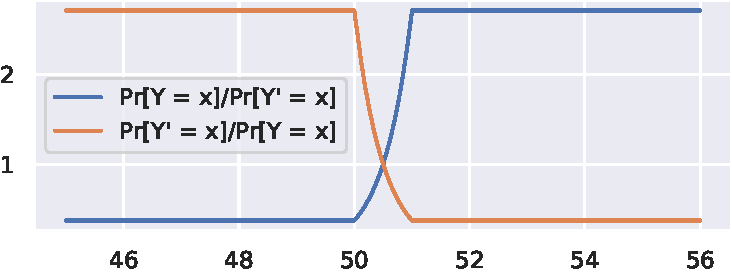
\includegraphics[width=0.8\linewidth]{img/laplace-03.pdf}
	\end{figure}
	
	Seems like the maximum we can get is $2.718 = e = \exp(1)$
	
	%\begin{tikzpicture}[overlay, remember picture]
	%\node at (current page.north east)[ref] {
		%\fullcite{Voigt.Bussche.2017} \par};
	%\end{tikzpicture}
\end{frame}


\begin{frame}{Previously: How does that relate to the maximum privacy loss?}
	Recall: likelihood of any output (x-axis) coming from $D'$ as opposed do $D$ (and vice versa)
	
	\begin{figure}
		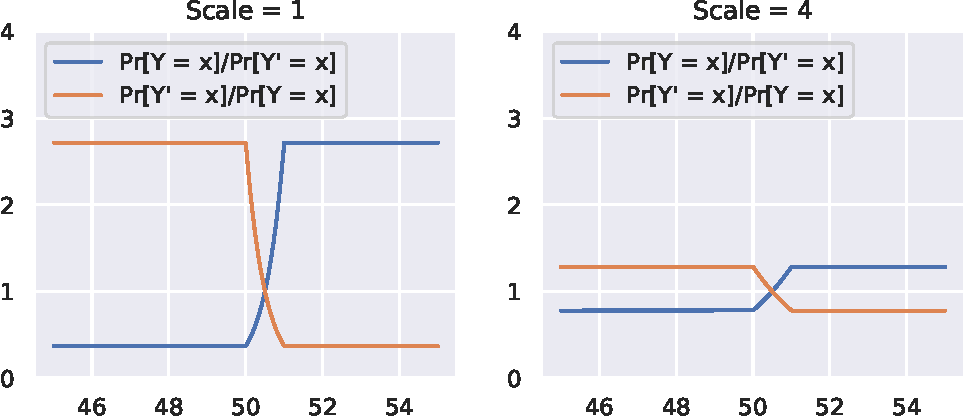
\includegraphics[width=0.8\linewidth]{img/privacy-loss1.pdf}
		\caption{Privacy loss for two Laplace distributions for a counting query, varying scale $b$}
	\end{figure}
	
\end{frame}

\begin{frame}{Recall: $(\varepsilon, 0)$ differential privacy (aka.\ pure DP)}
	
	A randomized algorithm (mechanism) $\mathcal{M}$ is $(\varepsilon, 0)$-\textbf{differentially private} if for any two neighboring datasets $D, D'$ and any output $\mathcal{Y} \subseteq \mathcal{Z}$ this guarantee holds:
	$$
	\Pr[\mathcal{M}(D) \in \mathcal{Y}] \leq \exp(\varepsilon) \Pr[\mathcal{M}(D') \in \mathcal{Y}]
	$$
	
	\begin{tikzpicture}[overlay, remember picture]
		\node at (current page.north east)[ref] {
			\fullcite[Definition~2.4]{Dwork.Roth.2013} \par};
	\end{tikzpicture}
	
\end{frame}


\begin{frame}{We bounded our `privacy loss' by $\varepsilon$}
\vspace{-1em}
$$
\begin{aligned}
\Pr[\mathcal{M}(D) \in \mathcal{Y}] &\leq \exp(\varepsilon) \Pr[\mathcal{M}(D') \in \mathcal{Y}] \\
\ln \left( \frac{
\Pr[\mathcal{M}(D) \in \mathcal{Y}]
}{
\Pr[\mathcal{M}(D') \in \mathcal{Y}]
}
\right)
&\leq \varepsilon
\end{aligned}
$$

What is $\mathcal{M}(D)$ (and also $\mathcal{M}(D')$)?

\pause

The private mechanism is randomized, so somewhere in the mechanism there is a random variable
\begin{itemize}
\item e.g., Laplace mechanism uses Laplace R.V.
\item Randomized response uses Bernoulli R.V., etc.
\end{itemize}
In general, since the mechanism $\mathcal{M}(D)$ is a function of a random variable, it is also a random variable

\end{frame}


\begin{frame}{Towards the `privacy loss' random variable}
$$
\ln \left( \frac{
\Pr[\mathcal{M}(D) \in \mathcal{Y}]
}{
\Pr[\mathcal{M}(D') \in \mathcal{Y}]
}
\right)
\leq \varepsilon
$$

$\mathcal{M}(D)$ (but also $\mathcal{M}(D')$) are random variables

\pause

In general, since the mechanism $\mathcal{M}(D)$ is a random variable, the entire left-hand side function
$
\ln \left( \frac{
\Pr[\mathcal{M}(D) \in \mathcal{Y}]
}{
\Pr[\mathcal{M}(D') \in \mathcal{Y}]
}
\right)
$
is again a random variable

(recall: random variables can be `pushed through' functions. If $X$ is a random variable, then $Y = g(X)$ is also a random variable. Here the $g$ is a complicated function even including probability of $X$)

\end{frame}




\begin{frame}{Step aside: You know functions of RV having similar form}
If $X$ is a discrete random variable

Expectation of $X$? \pause
$$
\mathbb{E}(X) = \sum_{x \in \text{Range}(X)} x \cdot \Pr[X = x]
$$
Entropy of $X$? (notice lazy notation for $P[X]$ and $\sum_x$)
$$
\mathbb{H}(X) = \mathbb{E}\left(\log \frac{1}{P[X]}\right) = 
- \sum_{x} x \cdot \log \Pr[X = x]
$$
\end{frame}


\begin{frame}{Step aside: You know functions of RV having similar form}
KL-Divergence between $X$ and $Y$ (same range)?
$$
\mathbb{D}(X || Y) = \mathbb{E} \left[
\log \frac{P(X)}{P(Y)}
\right]
$$

Here we implicitly assume $\log \frac{P(X)}{P(Y)}$ is a function of $X$ and is therefore distributed according to $X$
$$
\begin{aligned}
\mathbb{D}(X || Y) &= \mathbb{E} \left[
\log \frac{P(X)}{P(Y)}
\right]
= \mathbb{E}[g(X)] = 
\sum_{x \in \text{Range}(X)} \Pr[X = x] \cdot g(x) \\
&= \sum_{x \in \text{Range}(X)} \Pr[X = x] \log \frac{\Pr[X = x]}{\Pr[Y = x]} \\
\end{aligned}
$$
\end{frame}


\begin{frame}{Privacy Loss Random Variable}

$\mathcal{M}(D)$ and $\mathcal{M}(D')$ are two random variables

The privacy loss random variable is defined as
$$
\mathcal{L}_{\mathcal{M}(D) || \mathcal{M}(D')}
=
\ln \left( \frac{
\Pr[\mathcal{M}(D) = t]
}{
\Pr[\mathcal{M}(D') = t]
}
\right)
$$
and is distributed by drawing $t \sim \mathcal{M}(D)$

(Sanity check: You should know how to compute the expectation of the privacy loss R.V. given the previous slides)
\end{frame}

\begin{frame}{Example of Privacy Loss Random Variable}

\begin{block}{The privacy loss random variable}
$$
\mathcal{L}_{\mathcal{M}(D) || \mathcal{M}(D')}
=
\ln \left( \frac{
\Pr[\mathcal{M}(D) = t]
}{
\Pr[\mathcal{M}(D') = t]
}
\right)
$$
and is distributed by drawing $t \sim \mathcal{M}(D)$
\end{block}

How would the distribution of $\mathcal{L}_{\mathcal{M}(D) || \mathcal{M}(D')}$ would look like for the Laplace mechanism?
\begin{figure}
\centering
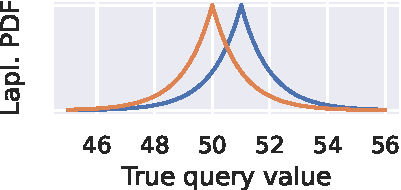
\includegraphics[width=0.5\linewidth]{img/laplace-pdfs-01.pdf}
\end{figure}

\end{frame}

\begin{frame}{Example of $\mathcal{L}_{\mathcal{M}(D) || \mathcal{M}(D')}$ for Laplace mechanism $\varepsilon = 1$}
\begin{figure}
\centering
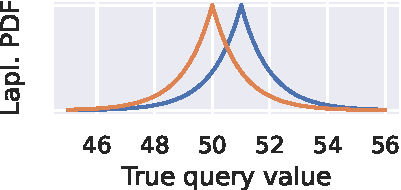
\includegraphics[width=0.4\linewidth]{img/laplace-pdfs-01.pdf}
\end{figure}

\begin{figure}
\centering
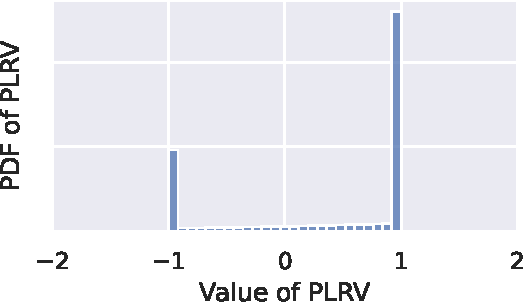
\includegraphics[width=0.6\linewidth]{img/loss1.pdf}
\end{figure}

\end{frame}


\begin{frame}{Values of $\abs{\mathcal{L}_{\mathcal{M}(D) || \mathcal{M}(D')}}$ are upper-bounded by $\varepsilon$ in $(\varepsilon, 0)$-DP}
\begin{figure}
\centering
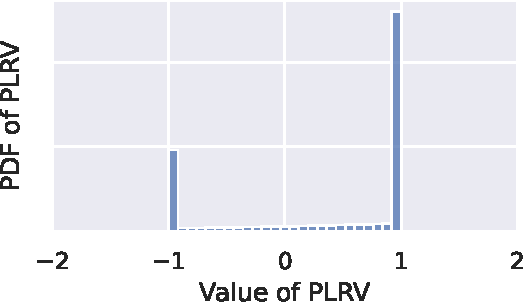
\includegraphics[width=0.5\linewidth]{img/loss1.pdf}
\end{figure}

This distribution demonstrates (not a proof!) that the probability the value of $\abs{\mathcal{L}_{\mathcal{M}(D) || \mathcal{M}(D')}}$ exceeds $\varepsilon$ is zero

In other words
$$
\Pr\left[\abs{\mathcal{L}_{\mathcal{M}(D) || \mathcal{M}(D')}} \leq \varepsilon \right]
= 1
$$

\end{frame}



\section{Approximate Differential Privacy}


\begin{frame}{Maybe we don't need to always ensure the bound}

What if we allow to exceed $\varepsilon$ with some small probability $\delta$?
\begin{figure}
\centering
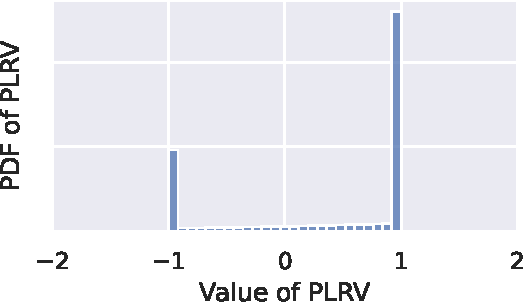
\includegraphics[width=0.5\linewidth]{img/loss1.pdf}
\end{figure}

In other words change $
\Pr\left[\abs{\mathcal{L}_{\mathcal{M}(D) || \mathcal{M}(D')}} \leq \varepsilon \right]
= 1
$
into
$$
\begin{aligned}
\Pr\left[\abs{\mathcal{L}_{\mathcal{M}(D) || \mathcal{M}(D')}} \leq \varepsilon \right]
&\geq 1 - \delta \\
\Pr\left[\abs{\mathcal{L}_{\mathcal{M}(D) || \mathcal{M}(D')}} > \varepsilon \right]
&< \delta \qquad \text{(equivalent)}
\end{aligned}
$$

\end{frame}


\begin{frame}{Formalizing approximate $(\varepsilon, \delta)$-DP}


A randomized algorithm (mechanism) $\mathcal{M}$ is $(\varepsilon, \delta)$-\textbf{differentially private} if for any two neighboring datasets $D, D'$ and any output $\mathcal{Y} \subseteq \mathcal{Z}$ this guarantee holds:
$$
\Pr[\mathcal{M}(D) \in \mathcal{Y}] \leq \exp(\varepsilon) \Pr[\mathcal{M}(D') \in \mathcal{Y}] + \delta
$$


One immediate observation: for $\delta = 0$ we get our known `pure' DP (that's why we called it $(\varepsilon, \delta)$-DP)

\begin{tikzpicture}[overlay, remember picture]
	\node at (current page.north east)[ref] {
		\fullcite[Definition~2.4]{Dwork.Roth.2013} \par};
\end{tikzpicture}

\end{frame}


\begin{frame}{Formalizing approximate $(\varepsilon, \delta)$-DP}
$$
\Pr[\mathcal{M}(D) \in \mathcal{Y}] \leq \exp(\varepsilon) \Pr[\mathcal{M}(D') \in \mathcal{Y}] + \delta
$$

This is equivalent to say\footnote{The proof is lengthy and technical, see \citet[pp.~44--47]{Dwork.Roth.2013}} that the P.L.R.V. is bounded by $\varepsilon$ with probability $1 - \delta$
$$
\Pr\left[\abs{\mathcal{L}_{\mathcal{M}(D) || \mathcal{M}(D')}} \leq \varepsilon \right]
\geq 1 - \delta
$$

\begin{tikzpicture}[overlay, remember picture]
	\node at (current page.north east)[ref] {
		\fullcite[Definition~2.4]{Dwork.Roth.2013} \par};
\end{tikzpicture}

\end{frame}


\section{What is this $\delta$ doing?}


\begin{frame}{Extreme algorithm 1: When bad things are really bad}
Our query is: Given a database of secrets, give me all rows

\begin{table}
\footnotesize
\begin{tabular}{lrrr} \toprule
Name & Hospitalized in year & Age & Illegal drug use \\ \midrule
Alice & 2024 & 32 & yes \\
Bob & 2020 & 21 & no \\
Charlie & 2023 & 45 & no \\
$\ldots$ & & & \\
Xander & 2020 & 31 & yes \\ \bottomrule
\end{tabular}
\caption{Example database $D$}
\end{table}

Our goal is to have this algorithm $(\varepsilon, \delta)$-DP

\end{frame}


\begin{frame}{Given a database of secrets, give me all rows (part 1)}

With probability $1 - \delta$, return completely random table

\begin{table}
\footnotesize
\begin{tabular}{lrrr} \toprule
Name & Hospitalized in year & Age & Illegal drug use \\ \midrule
Jim & 2022 & 16 & no \\
Dave & 2011 & 71 & yes \\
$\ldots$ & & & \\ \bottomrule
\end{tabular}
\caption{Example output of $\mathcal{M}(D)$ --- completely random}
\end{table}

Since the output is completely random, there would be no difference in outputs of any neighboring datasets $D$ and $D'$, therefore this is perfectly private algorithm $\varepsilon = 0$

\end{frame}


\begin{frame}{Given a database of secrets, give me all rows (part 2)}

With probability $\delta$, return the \textbf{original} dataset in full

\begin{table}
\scriptsize
\begin{tabular}{lrrr} \toprule
Name & Hospitalized in year & Age & Illegal drug use \\ \midrule
Alice & 2024 & 32 & yes \\
Bob & 2020 & 21 & no \\
$\ldots$ & & & \\ \bottomrule
\end{tabular}
\caption{Example output of $\mathcal{M}(D)$ --- returning the full original $D$}
\end{table}

This part of the algorithm is purely deterministic, there is no randomness, therefore this would be $\varepsilon = \infty$

\footnotesize{Why? Remove Alice to get $D'$. But this algorithm is never going to return $D'$, so $\Pr[\mathcal{M}(D') = 0]$, which leads to $\frac{\Pr[\mathcal{M}(D) = x]}{\Pr[\mathcal{M}(D') = 0]} \to \infty$}

\end{frame}

\begin{frame}{Given a database of secrets, give me all rows (part 3)}

Summary of our algorithm:
\begin{itemize}
\item With prob.\ $1 - \delta$, return completely random table ($\varepsilon = 0$)
\item With prob.\ $\delta$, return the \textbf{original} dataset in full ($\varepsilon = \infty$)
\end{itemize}
Our algorithm is $(\varepsilon, \delta)$-DP! (in fact $(0, \delta)$-DP)
$$
\Pr\left[\abs{\mathcal{L}_{\mathcal{M}(D) || \mathcal{M}(D')}} > \varepsilon \right] < \delta
$$

Very bad things can happen with $\delta$, so it should be very small! But how small?
\end{frame}



\begin{frame}{Extreme algorithm 2: Leak just a few rows}
Our query is: Given a database of secrets, give me a few rows verbatim

\begin{table}
\footnotesize
\begin{tabular}{lrrr} \toprule
Name & Hospitalized in year & Age & Illegal drug use \\ \midrule
Alice & 2024 & 32 & yes \\
Bob & 2020 & 21 & no \\
Charlie & 2023 & 45 & no \\
$\ldots$ & & & \\
Xander & 2020 & 31 & yes \\ \bottomrule
\end{tabular}
\caption{Example database $D$}
\end{table}

Our goal is to have this algorithm $(0, \delta)$-DP

\end{frame}

\begin{frame}{Extreme algorithm 2: Leak just a few rows}
Our algorithm 2:
\begin{itemize}
\item Iterate over all $n$ rows
\item For each row \textbf{independently}, with probability $\delta$ add this row to the output\footnote{For instance by drawing from $\mathrm{Ber}(\delta)$}
\end{itemize}
\begin{table}
\footnotesize
\begin{tabular}{lrrr} \toprule
Name & Hospitalized in year & Age & Illegal drug use \\ \midrule
Alice & 2024 & 32 & yes \\
Bob & 2020 & 21 & no \\
$\ldots$ & & & \\ \bottomrule
\end{tabular}
\caption{Example database $D$}
\end{table}

\end{frame}

\begin{frame}{Extreme algorithm 2: Leak just a few rows (part 2)}
Our algorithm 2:
\begin{itemize}
\item Iterate over all $n$ rows
\item For each row \textbf{independently}, with probability $\delta$ add this row to the output
\end{itemize}

This has again bad consequences!
Probability that at least one person will be leaked?\footnote{
Why? Pr.\ that a single person will not be leaked = $(1 - \delta)$. Pr.\ that no persons will be leaked = $(1 - \delta)^n$
}
$$
1 - (1 - \delta)^n \approx \delta n \qquad \text{for small }\delta
$$

\begin{footnotesize}

\end{footnotesize}
\end{frame}


\begin{frame}{Extreme algorithm 2: Leak just a few rows (part 3)}
Probability that at least one person will be leaked?
$$
1 - (1 - \delta)^n \approx \delta n \qquad \text{for small }\delta
$$

\begin{block}{General recommendation}
We should therefore consider
$$\delta \ll \frac{1}{n}$$
(ie.\ very small; typically $\delta = 1 \times 10^{-6}$, aka `cryptographically' small)
\end{block}

\begin{footnotesize}

\end{footnotesize}
\end{frame}

\section{Gaussian mechanism}


\begin{frame}{$\ell_2$ sensitivity}

Similar to $\ell_1$ sensitivity of the query

\begin{block}{$\ell_2$ sensitivity}
The $\ell_2$-sensitivity of a function $f : D \rightarrow \mathbb{R}^k$:

$$
\Delta_2 f = \max_{D, D'} \norm{f(D) - f(D')}_2
$$
\end{block}

\end{frame}

\begin{frame}{Gaussian (Normal) random variable}

The density (PDF) of a general univariate normal distribution $\mathcal{N}(\mu, \sigma^2)$

$$
f_X(x) =
\frac{1}{\sigma \sqrt{2\pi}} \exp \left(
- \frac{1}{2} \cdot \left( \frac{x - \mu}{\sigma} \right)^2
\right)
$$


\end{frame}


\begin{frame}{Gaussian mechanism}

Function (numeric query) $f : D \rightarrow \mathbb{R}^k$:

\begin{block}{Very important constraints on $\varepsilon$!}
For $\varepsilon \in (0, 1)$ and $\delta > 0$
\end{block}


The Gaussian mechanism $\mathcal{M}(D)$ is defined as
$$
f(D) + (Y_1, \ldots, Y_k)
$$
where each $Y_n$ is drawn \textbf{independently} from $\mathcal{N}(0, \sigma^2)$, such that
$$
%c^2 > 2 \ln (1.25 / \delta) \quad
%\sigma \geq c \Delta_2 / \varepsilon
%\quad
%\sigma^2 \geq c^2 (\Delta_2)^2 / \varepsilon^2
%\quad
%\sigma^2 > 2 \ln (1.25 / \delta) (\Delta_2)^2 / \varepsilon^2
\sigma^2 > 2 \ln \left( \frac{1.25}{\delta} \right) \frac{(\Delta_2)^2}{\varepsilon^2}
$$

\end{frame}

\begin{frame}{Gaussian mechanism is $(\varepsilon, \delta)$-DP\footnote{Non-trivial proof in Appendix~A of \citet{Dwork.Roth.2013}; also note that there are quite a few typos there}}

\begin{figure}
\centering
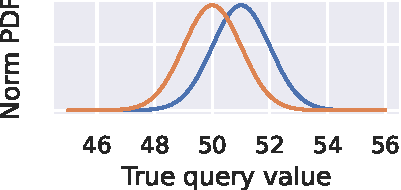
\includegraphics[width=0.45\linewidth]{img/gaussian-pdfs-01.pdf}
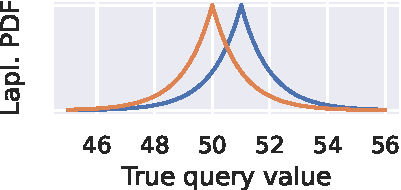
\includegraphics[width=0.45\linewidth]{img/laplace-pdfs-01.pdf}
\end{figure}


\begin{figure}
\centering
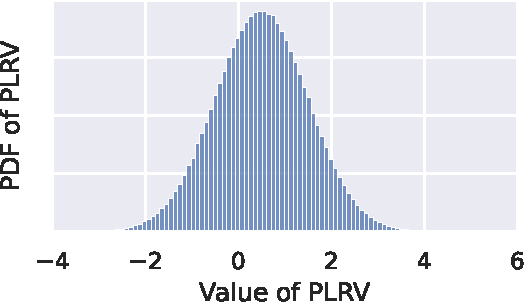
\includegraphics[width=0.45\linewidth]{img/loss2.pdf}
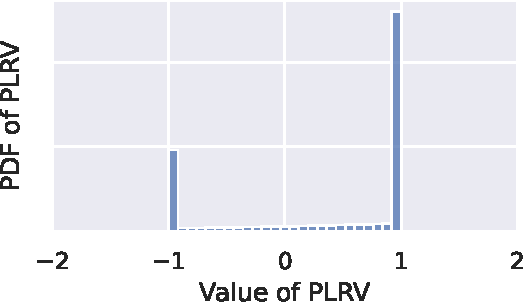
\includegraphics[width=0.45\linewidth]{img/loss1.pdf}
\end{figure}

\end{frame}

\section{General properties of DP algorithms}


\begin{frame}{Post-processing}

Let $\mathcal{M}(D) \mapsto R$ be a $(\varepsilon, \delta)$-DP algorithm

Let $f: R \mapsto S$ be an arbitrary (randomized) function

Then $f(\mathcal{M}(D))$ is $(\varepsilon, \delta)$-DP

\begin{block}{In words}
Whatever you do with $(\varepsilon, \delta)$-DP output, you cannot `weaken' privacy
\end{block}


\end{frame}


\begin{frame}{Group privacy}

Let $D$ and $D'$ differ in $k$ positions.

Let $\mathcal{M}(D)$ be $(\varepsilon, \delta)$-DP

Then for any output $T$ we have

$$
\Pr[\mathcal{M}(D) \in T] \leq \exp(k \varepsilon) \Pr[\mathcal{M}(D') \in T] +
k \exp(\varepsilon \cdot (k - 1)))
\delta
$$

\begin{block}{Implications for large groups}
If $k$ grows, the privacy budget grows exponentially
\end{block}

\end{frame}


\begin{frame}{Basic composition}

Let $\mathcal{M} = (M_1, \ldots, M_k)$ be a sequence of mechanisms, where each $M_i$ is $(\varepsilon_i, \delta_i)$-DP. (They might be adaptive)

Then $\mathcal{M}$ is $(\sum_{i = 1}^{k} \varepsilon_i, \sum_{i = 1}^{k} \delta_i )$-DP

\begin{block}{In words}
Overall privacy `budget' can be spent for a sequence of private queries
\end{block}

\end{frame}


\begin{frame}{License and credits}

	\begin{columns}
		\begin{column}{0.7\textwidth}
			Licensed under Creative Commons Attribution-ShareAlike 4.0 International (CC BY-SA 4.0)
		\end{column}
		\begin{column}{0.2\textwidth}
			
\includegraphics[width=0.9\linewidth]{img/cc-by-sa-icon.pdf}
		\end{column}
	\end{columns}
	
	\bigskip
	
	Credits
	
	\begin{scriptsize}
		
		Ivan Habernal
		
		Content from ACL Anthology papers licensed under CC-BY \url{https://www.aclweb.org/anthology}
		
		Partly inspired by lectures from Gautam Kamath
	
	\end{scriptsize}
	
\end{frame}



\end{document}

